\documentclass{article}
\usepackage[francais]{babel}
\usepackage[utf8]{inputenc} % Required for including letters with accents
\usepackage[T1]{fontenc} % Use 8-bit encoding that has 256 glyphs
\usepackage{pythontex}
\usepackage{amsthm}
\usepackage{amsmath}
\usepackage{amssymb}
\usepackage{mathrsfs}
\usepackage{graphicx}
\usepackage{geometry}
\usepackage{stmaryrd}
\usepackage{tikz}
\usetikzlibrary{patterns}
%\usetikzlibrary{intersections}
\usepackage[cache=false]{minted}

\usepackage{stmaryrd}
%\usepackage{tikz}
%\usetikzlibrary{tikzmark}
\usepackage{empheq}
\usepackage{longtable}
\usepackage{booktabs} 
\usepackage{array}
\usepackage{pstricks}
\usepackage{pst-3dplot}
\usepackage{pst-tree}
\usepackage{pstricks-add}
\usepackage{upgreek}
%\usepackage{epstopdf}
\usepackage{eolgrab}
\usepackage{chngpage}
 \usepackage{calrsfs}
 % Appel du package pythontex 
\usepackage{pythontex}

\usepackage{algorithm2e}
\RestyleAlgo{algoruled}
  \SetKw{KwFrom}{from} 
\newenvironment{algo}{
\begin{algorithm}[H]
\DontPrintSemicolon \SetAlgoVlined}
{\end{algorithm}}



\usetikzlibrary{decorations.pathmorphing}
\def \de {{\rm d}}
\usepackage{color}
\usepackage{xcolor}
\newcommand{\mybox}[1]{\fbox{$\displaystyle#1$}}
\newcommand{\myredbox}[1]{\fcolorbox{red}{white}{$\displaystyle#1$}}
\newcommand{\mydoublebox}[1]{\fbox{\fbox{$\displaystyle#1$}}}
\newcommand{\myreddoublebox}[1]{\fcolorbox{red}{white}{\fcolorbox{red}{white}{$\displaystyle#1$}}}

\usepackage{xcolor}
%\setbeamercolor{background canvas}{bg=lightgray}
\definecolor{LightGray}{gray}{0.9}

 \title{Les commandes}
\author{Ibrahim ALAME}
\date{14/02/2023}
\begin{document}
\maketitle
\section{Symfony CLI}
\begin{itemize}
\item Installez la commande symfony
\item Pour pouvoir utiliser HTTPS localement, nous avons également besoin
d’installer une autorité de certification pour activer le support TLS.
Exécutez la commande suivante :
\begin{verbatim}
> symfony server:ca:install
\end{verbatim}
\item Clonez le dépôt du livre d'or quelque part sur votre machine :
\begin{verbatim}
> symfony new --version=6.2-1 --book guestbook
\end{verbatim}
\item Exécuter en arrière plan:
\begin{verbatim}
symfony server:start -d
\end{verbatim}
\item Pour debugage:
\begin{verbatim}
dump($variable)
\end{verbatim}

\end{itemize}

\section{Routes}
La commande suivante  montre l'association
entre les noms de route et les chemins :
\begin{verbatim}
> symfony console debug:router
\end{verbatim}
\section{Doctrine}
Créer un {\tt User}:
\begin{verbatim}
symfony console make:user
\end{verbatim}
Créer une entité:
\begin{verbatim}
symfony console make:entity "Entité"
\end{verbatim}

\begin{itemize}
\item créer la base des données
\begin{verbatim}
symfony console doctrine:database:create
\end{verbatim}
\item  Migration
\begin{verbatim}
symfony console make:migration
\end{verbatim}
\item  Exécuter la migration générée pour mettre à jour
le schéma de la base de données locale :
\begin{verbatim}
symfony console doctrine:migrations:migrat
\end{verbatim}
\end{itemize}
\section{EasyAdmin}
\begin{itemize}
\item Ajoutez EasyAdmin comme dépendance du projet :
\begin{verbatim}
symfony composer req "admin:^4"
\end{verbatim}
\item Générer un “tableau de
bord d’administration” qui sera le point d’entrée principal pour gérer les données du site.
\begin{verbatim}
symfony console make:admin:dashboard
\end{verbatim}
\begin{center}
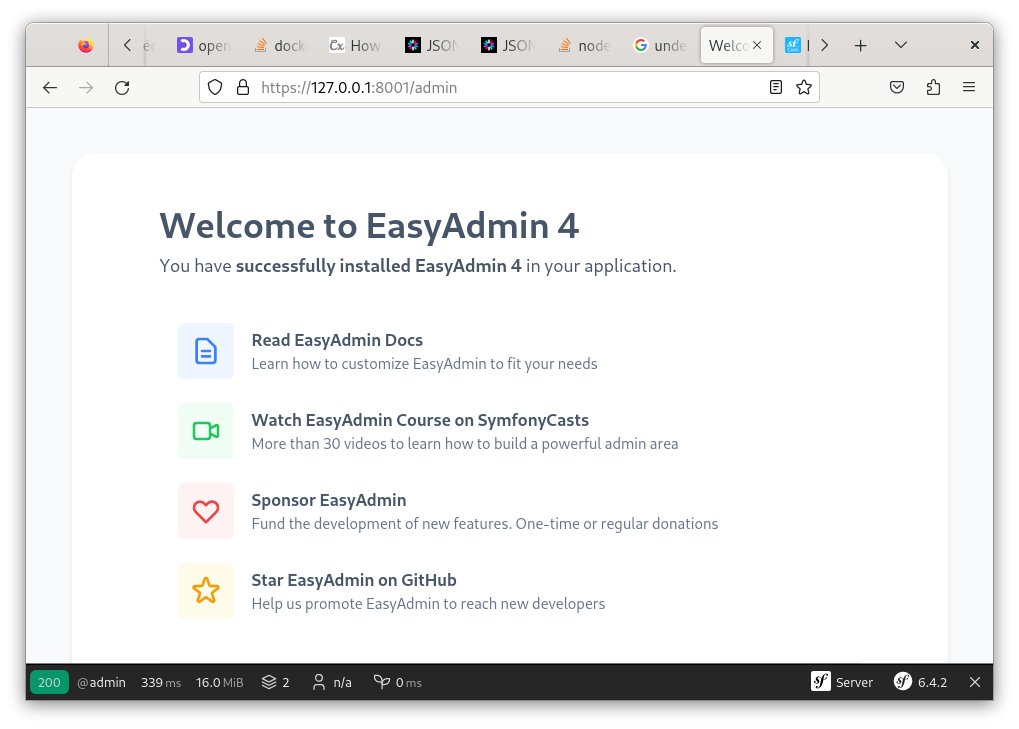
\includegraphics[width=15cm]{images/imageCommandes01.png}
\end{center}
\item Générer un CRUD  :
\begin{verbatim}
symfony console make:admin:crud
\end{verbatim}
\end{itemize}




\section{Git}
\begin{itemize}
\item création d'une branche Git :
\begin{verbatim}
git checkout -b sessions-in-db
\end{verbatim}
\end{itemize}



\section{Evenements}
\begin{itemize}
\item Implémenter un subscriber:
\begin{verbatim}
symfony console make:subscriber TwigEventSubscriber
\end{verbatim}

\end{itemize}

\section{Formulaire}
Générer un form type
Utilisez le Maker Bundle pour générer une classe de formulaire :
\begin{verbatim}
symfony console make:form CommentFormType Comment
\end{verbatim}


\section{Admin}
créer l’entité Admin au lieu de
la commande traditionnelle {\tt make:entity :}
\begin{verbatim}
symfony console make:user Admin
\end{verbatim}
générer une migration et de migrer la base de données :
\begin{verbatim}
> symfony console make:migration
> symfony console doctrine:migrations:migrate -n
\end{verbatim}
choisissez ce que vous voulez comme
mot de passe et exécutez la commande suivante pour générer le hash du mot de passe :
\begin{verbatim}
> symfony console security:hash-password
\end{verbatim}
Symfony accepte plusieurs stratégies
d’authentification. Utilisons un classique système d’authentification par formulaire. Exécutez la commande {\tt make:auth} pour mettre à jour la configuration de sécurité, générer un template pour la connexion et créer une classe d’authentification (authenticator) :
\begin{verbatim}
> symfony console make:auth
\end{verbatim}

\end{document}




